% !TEX program = xelatex

\documentclass[a4paper,11pt]{article}
\usepackage{xeCJK}

\usepackage{clrscode}

\usepackage{geometry}
\geometry{
 a4paper,
 left=30mm,
 top=30mm,
}
\usepackage[utf8]{inputenc}

\usepackage{graphicx}
\usepackage[english]{babel}
\usepackage{color}
\usepackage[dvipsnames]{xcolor}
\usepackage[colorlinks=true,urlcolor=blue,citecolor=black]{hyperref}
\usepackage{url}
%\urlstyle{same}
%\urlstyle{rm}
\urlstyle{sf}
%\urlstyle{tt}
\usepackage[font=footnotesize,labelfont=bf]{caption}
\usepackage[labelfont=it,textfont={it},singlelinecheck=on,justification=centering]{caption}
%full name for appendix
\usepackage[title]{appendix}
\usepackage{float}
\setlength{\parindent}{2em}
\usepackage{parskip}
%for code
\usepackage{listings}
%for math
\usepackage{amsmath}
\usepackage{breqn}
\usepackage{pdfpages}
\linespread{1.1}
\setlength{\emergencystretch}{3em}

\usepackage{ifxetex,ifluatex}
\usepackage{etoolbox}
\usepackage{tikz}

\usepackage{framed}

%water mark
\usepackage{eso-pic}

\newcommand{\watermark}[3]{\AddToShipoutPictureBG{
	\parbox[b][\paperheight]{\paperwidth}{
		\vfill%
		\centering%
	\tikz[remember picture, overlay]%
	  \node [rotate = #1, scale = #2] at (current page.center)%
	      {\textcolor{gray!80!cyan!30}{#3}};
	  \vfill}}}
\usepackage{blindtext}
%water mark end


% conditional for xetex or luatex
\newif\ifxetexorluatex
\ifxetex
  \xetexorluatextrue
\else
  \ifluatex
    \xetexorluatextrue
  \else
    \xetexorluatexfalse
  \fi
\fi
%
\ifxetexorluatex%
  \usepackage{fontspec}
  \usepackage{libertine} % or use \setmainfont to choose any font on your system
  \newfontfamily\quotefont[Ligatures=TeX]{STSong} % selects Libertine as the quote font
\else
  \usepackage[utf8]{inputenc}
  \usepackage[T1]{fontenc}
  \usepackage{libertine} % or any other font package
  \newcommand*\quotefont{\fontfamily{LinuxLibertineT-LF}} % selects Libertine as the quote font
\fi

\newcommand*\quotesize{60} % if quote size changes, need a way to make shifts relative
% Make commands for the quotes
\newcommand*{\openquote}
   {\tikz[remember picture,overlay,xshift=-4ex,yshift=-2.5ex]
   \node (OQ) {\quotefont\fontsize{\quotesize}{\quotesize}\selectfont``};\kern0pt}

\newcommand*{\closequote}[1]
  {\tikz[remember picture,overlay,xshift=4ex,yshift={#1}]
   \node (CQ) {\quotefont\fontsize{\quotesize}{\quotesize}\selectfont''};}

% select a colour for the shading
\definecolor{mygray}{gray}{0.95}
\colorlet{shadecolor}{mygray}

\newcommand*\shadedauthorformat{\emph} % define format for the author argument

% Now a command to allow left, right and centre alignment of the author
\newcommand*\authoralign[1]{%
  \if#1l
    \def\authorfill{}\def\quotefill{\hfill}
  \else
    \if#1r
      \def\authorfill{\hfill}\def\quotefill{}
    \else
      \if#1c
        \gdef\authorfill{\hfill}\def\quotefill{\hfill}
      \else\typeout{Invalid option}
      \fi
    \fi
  \fi}
% wrap everything in its own environment which takes one argument (author) and one optional argument
% specifying the alignment [l, r or c]
%
\newenvironment{shadequote}[2][l]%
{\authoralign{#1}
\ifblank{#2}
   {\def\shadequoteauthor{}\def\yshift{-2ex}\def\quotefill{\hfill}}
   {\def\shadequoteauthor{\par\authorfill\shadedauthorformat{#2}}\def\yshift{2ex}}
\begin{snugshade}\begin{quote}\openquote}
{\shadequoteauthor\quotefill\closequote{\yshift}\end{quote}\end{snugshade}}


\usepackage{listings}
\lstdefinestyle{myListStyle}{
  numbers=left,
  stepnumber=1,
  numbersep=10pt,
  tabsize=2,
  showspaces=false,
  showstringspaces=false
}

\usepackage[dvipsnames]{xcolor}
\usepackage{listings}

\newcommand\YAMLcolonstyle{\color{darkgray}\mdseries}
\newcommand\YAMLkeystyle{\color{black}\bfseries}
\newcommand\YAMLvaluestyle{\color{gray}\mdseries}

\makeatletter

% here is a macro expanding to the name of the language
% (handy if you decide to change it further down the road)
\newcommand\language@yaml{yaml}

\expandafter\expandafter\expandafter\lstdefinelanguage
\expandafter{\language@yaml}
{
  keywords={true,false,null,y,n},
  keywordstyle=\color{darkgray}\bfseries,
  basicstyle=\YAMLkeystyle,                                 % assuming a key comes first
  sensitive=false,
  comment=[l]{\#},
  morecomment=[s]{/*}{*/},
  commentstyle=\color{black}\ttfamily,
  stringstyle=\YAMLvaluestyle\ttfamily,
  moredelim=[l][\color{orange}]{\&},
  moredelim=[l][\color{magenta}]{*},
  moredelim=**[il][\YAMLcolonstyle{:}\YAMLvaluestyle]{:},   % switch to value style at :
  morestring=[b]',
  morestring=[b]",
  literate =    {---}{{\ProcessThreeDashes}}3
                {>}{{\textcolor{red}\textgreater}}1
                {|}{{\textcolor{red}\textbar}}1
                {\ -\ }{{\mdseries\ -\ }}3,
}

% switch to key style at EOL
\lst@AddToHook{EveryLine}{\ifx\lst@language\language@yaml\YAMLkeystyle\fi}
\makeatother

\newcommand\ProcessThreeDashes{\llap{\color{cyan}\mdseries-{-}-}}



%opening
\title{\LARGE Qitmeer 白皮书\\
	\Large 信任守护者}
\author{
	Qitmeer 团队\\
		\small\href{mailto:paper@qitmeer.io}
			{\nolinkurl{paper@qitmeer.io}}
	}
\date{\today\\\small Version 0.6.5}
\begin{document}

%% Cover end
\clearpage
\pagestyle{plain}

\maketitle

%\watermark{60}{10}{qitmeer.io}

\begin{abstract}
比特币\cite{bitcoin}与生俱来就带着革命的血液, 开创了以加密学为基础的更开放、更公平去中心化的新一代支付网络. 区块链作为比特币底层账本技术, 因其防篡改的特性, 能够在金融领域发挥关键的作用. 区块链将重塑普惠和伦理金融, 成为全球金融系统里面至关重要的一部分.

比特币诞生的十年以来, 区块链的基础设施正面临许多技术上的挑战. Qitmeer 坚持将开放性, 公平性, 容错性, 可伸缩性作为优质区块链的核心指标, 我们认为满足以上指标为经典区块链设定.

BlockDAG (区块图) 是一种高吞吐的框架, 以完全去中心化以及高安全性闻名. Qitmeer共识采用最先支持交易全排序的 BlockDAG 协议GhostDAG作为基础协议, 同时集成了SPECTRE保证交易的快速确认. Qitmeer 共识遵循经典区块链设定: 节点通过工作量证明可以自由进入和退出网络, 基于DAG账本的合作模型矿工可以根据自己的贡献公平地获得相应的回报, 于比特币相当的50\%算力安全性, 只受网络物理特性限制的强健的可伸缩性. 作为共识算法之外的重要公平性来源, Qitmeer 采用的布谷鸟环是一种基于图理论的工作量证明的挖矿算法因强内存依赖能有效地抗ASIC. 

出于合规的考虑, Qitmeer 设计了基于UTXO的独特的发币极致, 可以有效地应对两大挑战: 固有价值以及资产认证. 发布一定量的资产必须消耗等量的本币, 此外, 发布方必须被授予牌照.

Qitmeer 设计一系列规范与协议以融入全球普惠和伦理金融生态, 例如钱包以及矿工. Qitmeer 利用跨链协议以集成多种加密货币并提供可靠的智能合约服务.

\end{abstract}

\section{介绍}

\subsection{背景}

信任是金融系统的基石, 在传统途径中, 多个互不熟知的个体需要一个可信的第三方来保证交易的安全. 然和, 这个第三方是中心化的, 存在单点故障风险, 很难保证他的诚实.


比特币是一个开放的点对点网络, 意味着不存在一个中心化的服务器, 每个节点可以自由地加入或者退出网络. 计算复杂, 验证简单的工作量证明共识被设计成保证节点能获得与其贡献相应的回报, 本应是一种公平的机制. 比特币采用类似散列表结构的账本以保证防篡改, 这种颠覆式的设计驱动着大量对于其机制的研究. “区块链”的概念就是后被引入来表示这种机制并被广泛接受. 由于免信任以及防篡改的特性, 越来越多的区块链应用涌现在金融领域并成为驱动金融系统重塑的全新动力.

比特币的十年前的创新以来, 区块链的基础设施一直面临着众多技术上的挑战并偏离其哲学的本质. 比特币不再去中心化, 前五大矿池已经控制了大多数的算力使得他们在有必要的情况下可以轻松地攻击网络. 矿工必须加入矿池因为在同等收益期望的情况下可以降低风险. 换言之, 比特币不在公平了. 此外, 比特币不可伸缩, 7笔每秒的吞吐量, 一小时的确认时间, 高昂的交易费, 作为全球支付网络来说很难说是一个令人满意.

比特币需要革新以反映其哲学的本质. 无数种方案声称已经解决了这些挑战. 然而真正做到的并不多, 一般都是牺牲某一种特性而换取另一种特性, 如牺牲去中心化, 安全性的核心来源来换取可伸缩性. 因此, 比特币的哲学本质是什么? Qitmeer 定义其为经典区块链设定, 并深刻启发着Qitmeer网络的设计哲学. 


\subsection{经典区块链设定}
有许多区块链的变种, 各自有各自对区块链的定义.  Qitmeer 网络认可比特币的, 认为如下四种指标为经典区块链设定.

\subsubsection{开放性}
开放性是区分许可链和非许可链的本质特性, 意味着每个节点应该能自由地加入和退出网络.

一个开放的网络应该允许不同的角色, 在比特币网络中, 节点可以自由选择成为SPV (简化支付验证) 节点, 全节点或者矿工, 所以从协议的角度来讲比特币是开放的. 而其他某些共识, 例如, 在代理权益证明中, 区块生产者是根据预定的配置, e.g., 21 个生产者, 在链外被选举产生, 因而限制了网络的开放性.

\subsubsection{公平性}
公平性意味着在一个激励相融的系统中, 回报应该和贡献匹配

\subsubsection*{挖矿风险}
从概率的角度而言, 独立挖矿与加入矿池挖矿的期望收益是相同的, 但是独立挖矿的风险是相当高的, 即要么获得巨额的奖励要么就是长时间得不到任何回报. 因此, 矿工不得不加入矿池以获得稳定的激励. 

\subsubsection*{挖矿效率}
挖矿成本主要包含电力价格以及挖矿效率, 而后者因为ASIC矿机更加关键. ASIC 被定制用于执行特定挖矿算法, 所以单位成本挖矿效率要远高于通用计算机. 例如, 蚂蚁矿机S9 的效率要高出GTX570 两万倍; 个人计算想要参与挖矿竞赛几乎是不可能的. 

\subsubsection{安全性}
安全性是指网络在遭受攻击时的健壮程度. 一般是指推翻一笔确认了的交易


\subsubsection*{去中心化}
去中心化相对于传统支付网络来说是最关键的特性. 去中心化可以规避单点故障, 因为要串通一个去中心化网络中的大部分节点几乎是不可能的.

\subsubsection*{容错性}
容错指网络应该可以承受失效节点的最大比例. 在去中心化网络中, 根据少数服从多数的原则, 50\%的算力容错性是最理想的比例.

\subsubsection{可伸缩性}
随着规模的增长, 网络如果仍能够提供相对稳定增长的服务则可以被认为是可伸缩的. 这些服务包括:
\subsubsection*{吞吐量}
吞吐量是指每秒的交易数, 当网络在扩张时其性能至关重要. 而迄今为止, 比特币当吞吐量仍然限定在七笔每秒, 无论网络有多少节点. 因而限制其成为全球支付网络.

\subsubsection*{确认时间}

确认时间是指接收方需要等待交易不容易被推翻所需的时间, 该时间不应该随着网络规模的增大而增加.  在比特币网络, 确认时间长达六个区块或者一个小时. 确认时间非常影响支付的体验, 例如, 比特币的确认时间是六个区块或一个小时, 一般用户很难接受.

\subsubsection*{成本}

交易费是成本的主要部分, 应该要维持在一个相对合理的范围, 因为如果交易费过高, 支付就不再实用, 而如果过低则容易遭受女巫攻击. 比特币的交易费变得越来越高, 已经不再适合作为原本想成为的全球支付网络. 至目前为止, 比特币的平均交易费大概有两美元之多.

\subsection{设计规范}
Qitmeer 的设计规范遵循经典区块链设定. 这四个指标彼此之间存在内在的矛盾, Qitmeer 不可能同时让每个指标都达到最优, 而是找到一个最佳都平衡, 即在满足公平性和安全性都情况下, 尽可能高地提高可伸缩性.

\subsubsection{开放性}

\subsubsection*{工作量证明}
工作量证明是最开放的加入区块链网络的途径, 因为只需要电力就可以加入, 而电力是一人人都拥有的物理资源. 
\subsubsection*{无预定节点}
预定节点是指协议定义的特殊节点. 注意, 尽管存在矿池这样特殊的节点, 但是它们属于协议之外的产物. 因而, 比特币也是无预定节点的, Qitmeer 在这方面是遵循比特币的规范的, 所以也不存在预定的特殊节点.
\subsubsection{公平性}
BlockDAG 是公平的因其引入的合作模型替代区块链的竞争模型.

\subsubsection*{矿池去中心}
竞争模型会导致收益波动的挖矿风险, 进而导致矿池的中心化. Qitmeer 共识协议基于合作模型的BlockDAG框架, 独立可以和矿池挖矿一样处于低风险水平, 所以矿池也会更去中心化.

\subsubsection*{抗ASIC的挖矿算法}
布谷鸟环是一个基于图理论的工作量证明算法, 因其抗ASIC的特性而流行. Qitmeer 采用这个算法以保证没有哪个矿工可以有过高的挖矿效率.
\subsubsection{安全性}
安全性是Qitmeer网络最重要的考虑因素. Qitmeer已经达到了完全的去中心化以及50\%的算力容错性. 因此, Qitmeer并没有牺牲安全性来获得其他指标的性能.
\subsubsection*{完全去中心化}
Qitmeer网络的所有节点都是对等节点并有资格参与共识. 

\subsubsection*{50\% 容错性}
恶意节点必须拥有50\%的算力才能控制整个网络. Qitmeer 共识的容错性与吞吐量无关, 无论吞吐量多高依然保持相同的容错性, 而比特币的容错性跟吞吐量是负相关的.

\subsubsection{可伸缩性}
Qitmeer 在各种可伸缩性的方面都有理想的表现, 使得它能长时间稳定运行.

\subsubsection*{快速确认}
Qitmeer 集成SPECTRE, 一个高速确认的BlockDAG协议, 来保证交易的快速安全确认.
\subsubsection*{高吞吐量}
GhostDAG 是一个支持高吞吐量的BlockDAG协议, 能充分发掘潜在的伸缩性, 只受网络物理参数的限制, 例如网络带宽或传播时间.

\subsubsection*{低成本}
技术上讲, 成本不能扩张因为交易费会随着网络的增长缓慢地增长.不过平均每笔交易的成本还是相对不是太显著, 长远看还是合理的.


\section{Qitmeer 通证设计}

当前的区块链网络, 在开始项目设计的时候, 完全没有考虑到合规性以及道德关切. 相较而言, Qitmeer 将合规性根植在从底层逻辑, 并贯穿在整个技术架构, 直至生态应用. 在此过程中, Qitmeer 设计了一套有效都方案, 称之为OP_TOKEN.

\subsection{背景}
\subsubsection{问题定义}

区块链的合规性应该要考虑两点:

\subsubsection*{内在价值}

资产必须存在内在价值, 不能凭空产生. 在已有的通证发布平台例如以太\cite{Ethereum}, 个人可以在不需要抵押的情况下发布任意额度的资产
 

\subsubsection*{资产认证}
区块链不应该允许非法资产的发行以及违反商业操守的行为, 已有的区块链在资产认证时没有任何限制. 

\subsubsection{相关工作}

$\texttt{OP\_TOKEN}$ 的设计灵感来源于染色币, 基于比特币的 $\texttt{OP\_RETURN}$ 和  OP\_GROUP  用于代表并管理现实生活中的资产, 其中 OP\_GROUP 是一个Andrew Stone实现的用于发行资产的参考实现, 

\subsubsection*{UTXO}

UTXO 即未花费的交易输出, UTXO用于判断一笔交易是否是合法, 在Qitmeer 网络中并不存在账号. 用户花费的是一组UTXO. 通过求和UTXO可以得到总余额.

\begin{figure}[hbt]
	\centerline{%
	   \resizebox{0.8\textwidth}{!}{\includegraphics{figures/UTXO}}%
	}
\caption{UTXO 模型}
\end{figure}

交易1 tx1 有两笔UTXO(绿色), 所以tx1有2+3=5 个币的余额.

交易2 花费了 tx1的两笔UTXO, 并支付到了三个地址, 产生了三笔新的UTXO.

注意: 现在就的UTXO (tx1的) 已经不在是UTXO了, 所以不能再被花费了.

\subsubsection*{脚本系统}

花费UTXO的机制其实就是执行一段脚本. 输出存储了一半的脚本并必须出具另外一半脚本并合并两者以验证该笔金额是否可以被花费. 前一部分称为锁定脚本, 就像一个锁住的宝箱, 后半部分叫解锁脚本, 就像该箱子唯一的钥匙.

例如, UTXO 中一段典型的 "支付到公钥哈希" (Pay-2-Public-Key-Hash(P2PKH)\cite{P2PKH}) 锁定脚本:

\begin{lstlisting}
OP_DUP OP_HASH160 <PUBLIC_KEY> OP_EQUALVERIFY OP_CHECKSIG
\end{lstlisting}

一笔新建交易的解锁脚本

<Signature><PublicKey>

将锁定脚本和解锁脚本合并

<Signature><PublicKey> OP\_DUP OP\_HASH160 <PUBLIC\_KEY> OP\_EQUALVERIFY OP\_CHECKSIG

完整的脚本包含两个步骤:
1. <PublicKey>  OP\_HASH160 <PUBLIC\_KEY> OP\_EQUALVERIFY
	验证解锁脚本中的公钥是否匹配锁定脚本中的私钥
2.  <Signature><PublicKey> OP\_CHECKSIG
	检查签名是否是合法的

\subsubsection*{染色币 和 Tether}

染色币\cite{ColoredCoins} 是一套在区块链上表示资产的方法, 它可以利用区块链防篡改的能力. 它使用${OP\_RETURN}$中断脚本的执行, 因此, 它可以在$\texttt{OP\_RETURN}$ 后面加协议内容而并不需要违反脚本的验证.

锁定脚本:
\begin{lstlisting}
OP_RETURN <DATA>
\end{lstlisting}

此外, 稳定币 Tether\cite{Tether} (USDT) 也使用了基于 OP\_RETURN 的OMNI Layer 协议来定义比特币上的资产.

典型的USDT交易以及协议设计的详细内容

\lstset{basicstyle=\tiny,style=myListStyle}
\begin{lstlisting}
OP_RETURN 6f6d6e69000000000000001f00000015c9054900
\end{lstlisting}


\begin{figure}[hbt]
	\centerline{%
	   \resizebox{0.8\textwidth}{!}{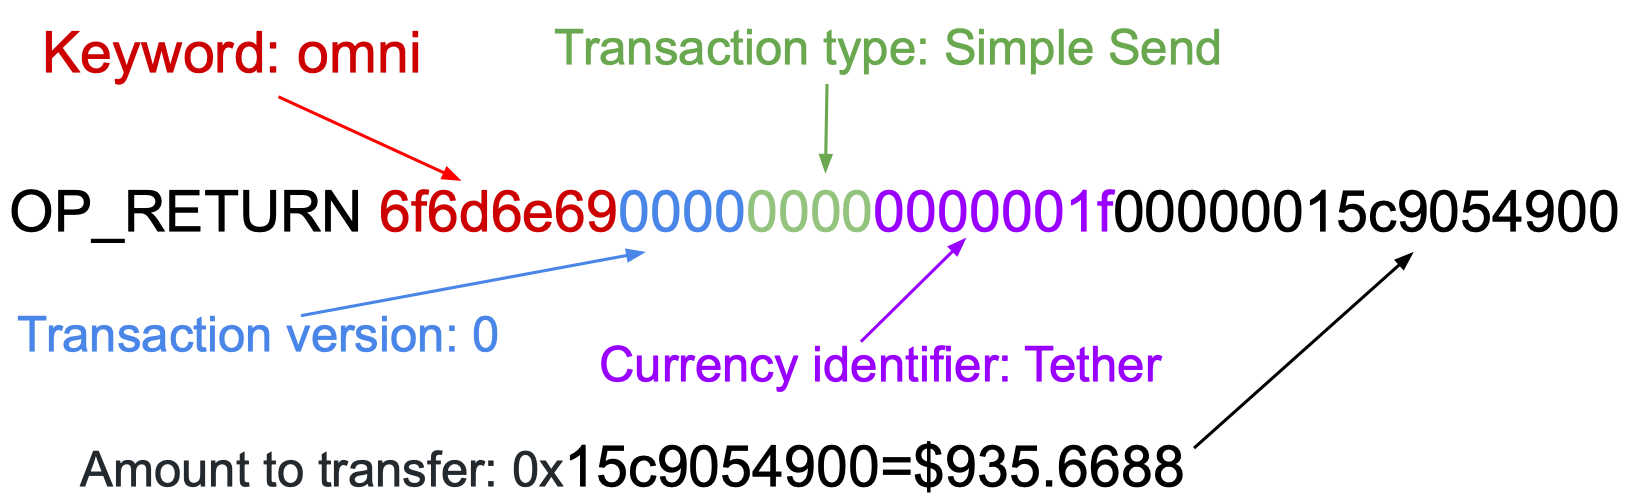
\includegraphics{figures/USDT}}%
	}
\caption{USDT}
\end{figure}


%[ref][https://www.blockchain.com/btc/tx/efc50d9e1f23e687e304cfca4ef2c5412b67d5737888ff80a0cbb6853cd865c]


\subsubsection*{OP\_GROUP}
OP\_RETURN 的设计更适合在成熟的区块链上应用, 因为它不会改变底层区块链协议, 从而不会有分叉的风险. 不过缺点在于矿工是无法验证协议, 所以可能存在一定的安全风险.

OP\_GROUP\cite{OP_GROUP} 是Bitcoin Unlimited (BU) 提出的针对比特现金\cite{BCH}的提案. 因此, OP\_GROUP 支持转账, 销毁以及发行通证. 因为OP\_GROUP是对BCH 脚本系统的扩展, 它是属于协议的一部分	 


基本的“染色”支付到公钥散列脚本应该是:

\lstset{basicstyle=\tiny,style=myListStyle}
\begin{lstlisting}[numbers=none]
OP_DATA(group address)
OP_GROUP
OP_DROP
OP_DUP
OP_HASH160
OP_DATA(pubkeyhash)
OP_EQUALVERIFY
OP_CHECKSIG
\end{lstlisting}

主要的区别很简单,只是添加一个组地址来区分不同的组,而其他操作,例如创建和销毁资产,是类似的。

% [ref]https://medium.com/@g.andrew.stone/bitcoin-scripting-applications-representative-tokens-ece42de81285

\subsection{OP\_TOKEN 设计}

\subsubsection{概述}


在OP\_TOKEN中有一个名为牌照(LICENSE)的惟一通证。相关监管实体、在生态系统中具有公信力的行业从业人员将被邀请领取牌照,以监督在主流采用协议过程中可能出现的遵从性问题。任何计划发布令牌的实体都需要获得许可。对等点可以传输许可证,因为它们本身也是令牌。然而,发端人在转移时必须格外小心,以避免由于记录是公开和不可变的而造成的不遵从风险。

在OP\_TOKEN中有一个名为牌照或者许可证(LICENSE)的惟一通证。在生态系统中具有公共信誉的相关监管实体和行业从业人员被邀请领取许可证,以管理可能发生的合规性问题。任何计划发布通证的实体都需要获得许可。对等节点之间可以传输许可证,因为它们本身也是通证。由于记录是公开的、不可变的,为了避免向错误的人转移的不合规风险,发起者在转移时必须格外小心。
 

\subsubsection{许可证生成}


许可证都是在创世块中生成的,并分发给C名保护委员会成员。
一个最小的单位(QIT)可以代表一个许可证,一个块有M个本币,1个本币= N个QIT,所以我们总共有M*N个许可证,这就足够发行资产了。


\begin{lstlisting}[language=yaml, numbers=none,basicstyle=\footnotesize]
# C = 100, M = 10, N = 10^8 (M*N = 100 亿),
# 所以的示例都基于这组参数 
# 例1: 分发牌照给委员会,
# M*N/C = 100,000,000, 分配给每个委员一亿个牌照.
---
INPUTS:
	INPUT:
		PREVIOUS_OUTPUT: # (创世 COINBASE )
			S: "DUP HASH160 [GEN] EQUALVERIFY CHECKSIG"
			V: 10000000000
		S: "[SIG] [GEN_PK]"
OUTPUTS:
	OUTPUT:
		S: "[LIC] TOKEN DROP DUP HASH160 [COMM1] EQUALVERIFY CHECKSIG"
		V: 100000000
	# ... ... (COMMITTEE MEMBER 2~99)
	OUTPUT:
		S: "[LIC] TOKEN DROP DUP HASH160 [COMM100] EQUALVERIFY CHECKSIG"
		V:100000000
	OUTPUT:
		S: "RETURN [DATA]"
		V: 0
\end{lstlisting}



\subsubsection{颁发许可证}


相关实体必须获得授权才能发行资产。
实体可以向任何委员会成员(C.M.)申请许可证。
一旦许可被授予和批准。
这些实体将从委员会成员接收一个特定的,该令牌是经过许可的。

\lstset{basicstyle=\tiny,style=myListStyle}
\begin{lstlisting}[language=yaml, numbers=none,basicstyle=\footnotesize]
# 例2:  委员会颁发证书给发行方 (ISS),
# 注意许可证的余额会返还到委员会.
---
INPUTS:
	- INPUT:
			PREVIOUS_OUTPUT:
				S: "[LIC] TOKEN DROP DUP HASH160 [COMM] EQUALVERIFY CHECKSIG"
				V: 100000000
			S: "[SIG] [COMM_PK]"
OUTPUTS:
	- OUTPUT:
			S: "[LIC] TOKEN DROP DUP HASH160 [ISS] EQUALVERIFY CHECKSIG"
			V: 1
	- OUTPUT: # License change
			S: "[LIC] TOKEN DROP DUP HASH160 [COMM] EQUALVERIFY CHECKSIG"
			V: 99999999
	- OUTPUT:
			S: "RETURN [DATA]"
			V: 0
\end{lstlisting}

\subsubsection{资产发行}
一旦获得授权,实体就可以发行资产;但是,他们不能任意设置通证数量。相反,发行一定数量的资产需要转换相同数量的QIT。Qitmeer网络将这个过程称为“铸币”。就像现实中的情况一样,铸造一枚金币需要同样重量的金币,代币需要同样数量的金币。

发行制度的首要优点是保证了代币的基本内在价值;因此,它将大大缓解价格波动。另一个好处是,代币和本币不再是价值孤岛,它们在同一个生态系统中运行,将提高流动性,使整个网络稳定

\lstset{basicstyle=\tiny,style=myListStyle}
\begin{lstlisting}[language=yaml, numbers=none,basicstyle=\footnotesize]
# 例3: 转换 100000000 QIT, 即 1 MEER,
# 到 100000000 单位的新通证,
# 注意:许可证将返回给发行方以备将来发行
INPUTS:
	- INPUT:
			PREVIOUS_OUTPUT: #(1 LICENSE)
				S: "[LIC] TOKEN DROP DUP HASH160 [ISS] EQUALVERIFY CHECKSIG"
				V: 1
			S: "[SIG] [LIC_PK]"
	- INPUT:
			PREVIOUS_OUTPUT: #(1 Qitmeer Coin)
				S "DUP HASH160 [COIN] EQUALVERIFY CHECKSIG"
				V: 100000000
			S: "[SIG] [COIN_PK]"
OUTPUTS:
	- OUTPUT: # License returns to the issuer
			S: "[LIC] TOKEN DROP DUP HASH160 [ISS] EQUALVERIFY CHECKSIG"
			V: 1
	- OUTPUT:
			S: "[TOK] TOKEN DROP DUP HASH160 [PK] EQUALVERIFY CHECKSIG"
			V: 100000000
	- OUTPUT:
			S: "RETURN [DATA]"
			V: 0
\end{lstlisting}

\subsubsection{资产转移}

实体之间可以相互转移资产。
此外,实体可以在一个交易中转移多个资产。
交易需要确保每个资产的输入和等于每个资产的输出和

\lstset{basicstyle=\tiny,style=myListStyle}
\begin{lstlisting}[language=yaml, numbers=none,basicstyle=\footnotesize]
# 例4: Alice 用 Bob 的20美元代币兑换她的100元人民币代币。
INPUTS:
	- INPUT:
			PREVIOUS_OUTPUT:
				S: "[RMB] TOKEN DROP DUP HASH160 [A_PKH] EQUALVERIFY CHECKSIG"
				V: 100
			S: "[A_SIG] 0X83 [A_PK]"
	- INPUT:
			PREVIOUS_OUTPUT:
				S: "[USD] TOKEN DROP DUP HASH160 [B_PKH] EQUALVERIFY CHECKSIG"
				V: 20
			S: "[B_SIG] 0X83 [B_PK]"
OUTPUTS:
	- OUTPUT:
			S: "[USD] TOKEN DROP DUP HASH160 [A_PKH] CHECKSIG"
			V: 20
	- OUTPUT:
			S: "[RMB] TOKEN DROP DUP HASH160 [B_PKH] CHECKIG"
			V: 100
\end{lstlisting}


\subsubsection{融币}

熔币是铸币的相反过程,即,从代币到本币的转换。无论是以本机qit还是令牌qit的形式,qit的总量都是常量。但是,它可以转换令牌和转换本地货币。发行方可以通过融币来降低流动性,以保持价格稳定,这对于稳定货币的实施是很现实的。令牌熔炼保证了令牌的基本价值,就像一枚金币的最小价值等于黄金的重量一样。

\lstset{basicstyle=\tiny,style=myListStyle}
\begin{lstlisting}[language=yaml, numbers=none,basicstyle=\footnotesize]
# 例5: 熔化 100 QIT 代币  到 100 QIT 本币 
INPUTS:
	- INPUT:
			PREVIOUS_OUTPUT:
				S: "[TOK] TOKEN DROP DUP HASH160 [ISS] EQUALVERIFY CHECKSIG"
				V: 100
			S: "[SIG] [ISS_PK]"
OUTPUTS:
	- OUTPUT:
			S: "DUP HASH160 [COIN] EQUALVERIFY CHECKSIG"
			V: 100
	- OUTPUT:
			S: "RETURN [DATA]"
		V: 0
\end{lstlisting}


\section{共识协议}

BlockDAG是一个高吞吐量的框架,亮点在于在完全去中心化和高安全性。
此外,它是对经典比特币范式的自然延伸,这意味着它将继承比特币最长久以来被验证的特性,并有望具有更强的稳定性。

Qitmeer引入GHOSTDAG作为基础协议,实现高吞吐量的线性排序服务,并采用SPECTRE协议保证快速确认

\subsection{从 区块链 到 区块图}
由于协议约束,比特币不可伸缩。根据中本聪共识,即,最长链规则,1 MB块大小和10分钟块率限制比特币只能达到每秒7笔交易的理论吞吐量,无论多么大的带宽和多么快的传播延迟。

提高可伸缩性最直观的方法是缩短块时间或增大块大小。中本聪没有采用的原因是这样会带来分叉,同时会分散主链的算力,从而造成安全漏洞。


GHOST协议在不牺牲安全性的前提下,引入了最重树共识来保留分叉。注意,这里区块链已经转换为块树。由于最大的子树集中了大多数算力,安全性与比特币一样高。主链是指从起源到子代数量最多的叶子上的区块链,其他区块为链下区块。只有主链块贡献吞吐量,而链下区块有助于增强安全性。

由于更高的出块速率或区块大小,区块树极大地提高了吞吐量。但是,仍然存在对链下块中交易的浪费,而这些交易也应该有助于提高吞吐量。Inclusive\cite{Inclusive} 协议提出了一种新的账本数据结构,即每一个区块确认每一个未确认的区块。此改进将块树升级为区块图。

从区块链到BlockDAG的发展历史可以看出,区块链是BlockDAG在低吞吐量情况下的一个特例,这意味着两者在本质上是相同的。因此,它是最接近比特币网络的可伸缩性解决方案。BlockDAG是健壮的,因为它继承了所有被长期证明是稳定的比特币的特点,并且它在协议层面可以无限地扩展,只有物理上的限制,如,带宽和传播延时。健壮的公共链是整合进一步扩展解决方案(如分片和状态通道)的最佳基础,因此BlockDAG是Qitmeer的首选扩展解决方案。


\begin{figure}[hbt]
	\centerline{%
	   \resizebox{0.8\textwidth}{!}{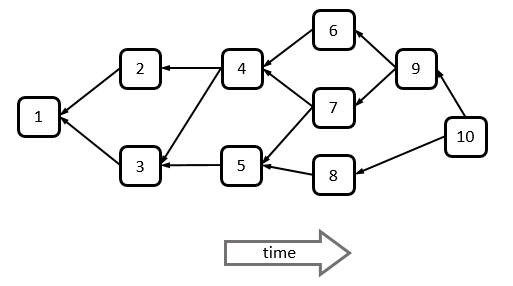
\includegraphics{figures/DAG.png}}%
	}
\caption{DAG}
\end{figure}

\subsection{GHOSTDAG}

GHOSTDAG,前身为Phantom,是第一个支持区块全序的BlockDAG协议。而且,与SPECTRE相比,它保证了强活性,即在一定时间内,诚实区块和恶意区块都可以被确认,这使得共识协议更加健壮。

\subsubsection{设计思想}

这是GHOSTDAG背后的想法。
假设网络传播时延和块生成的最大极限率是常数。
可以直观地看出,如果节点的行为是诚实的,那么它将形成一个子图,其中每个块最多拥有一个常数数量的分叉。
我们表示这个常数是$k$。
$k$可以从传播时间和出块率计算出来。
子图表示为$k$-集群。
最大的$k$-集群被称为蓝色集合。蓝色集合之外的那些块被称为红色集合.


如果我们可以通过跟随父块在每个块内的引用, 从$x$块遍历到$y$块,那么我们说在它们之间有一个偏序$x$和$y$, $y$在$x$之前。例如在下面的图中,我们可以从J块到A再到B,所以在A之间有一个偏序. 注意,并不是所有的块都与其他块有偏序。例如,在B、C和D之间不存在偏序。不存在偏序的区块集叫反锥体。$k$-集群中反锥体的大小最多是$k$。


\begin{figure}[ht]
	\centerline{%
	   \resizebox{0.8\textwidth}{!}{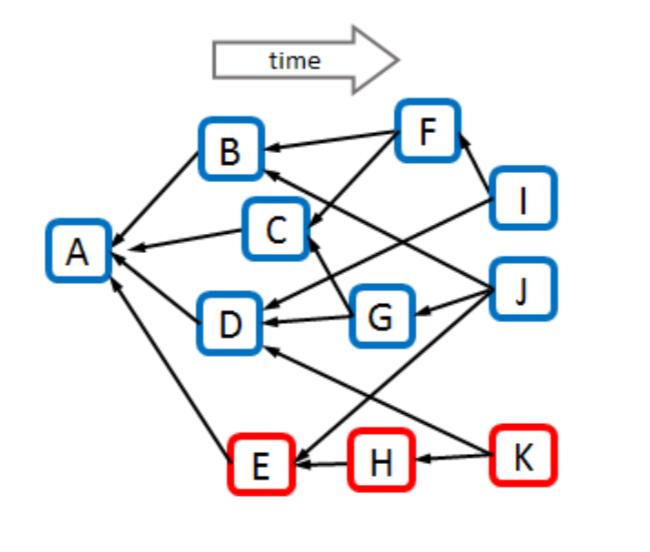
\includegraphics{figures/GHOSTDAG}}%
	}
\caption{GHOSTDAG}
\end{figure}


\subsubsection{排序}

GHOSTDAG以一种偏爱蓝色方块和惩罚红色块的方式来排序DAG账本。所以,如果两个方块X和Y在图上没有偏序,那么蓝色的那个在前面,红色的那个在前面。

着色算法是基于一个块的过去集,也称为祖先,因为在生成一个块后,过去集就确定下来了,所以蓝色的集合也会确定下来。因此,每个块可以选择最大蓝色集作为其主父块。然后,重复从末端块到创世块寻找主父块的过程,最后我们可以找到一个唯一的被大多数网络同意的区块链,我们将这个区块链命名为主链。一旦主链被确定,所有的块可以形成一个线性的顺序参考它。

\begin{figure}[ht]
	\centerline{%
	   \resizebox{0.8\textwidth}{!}{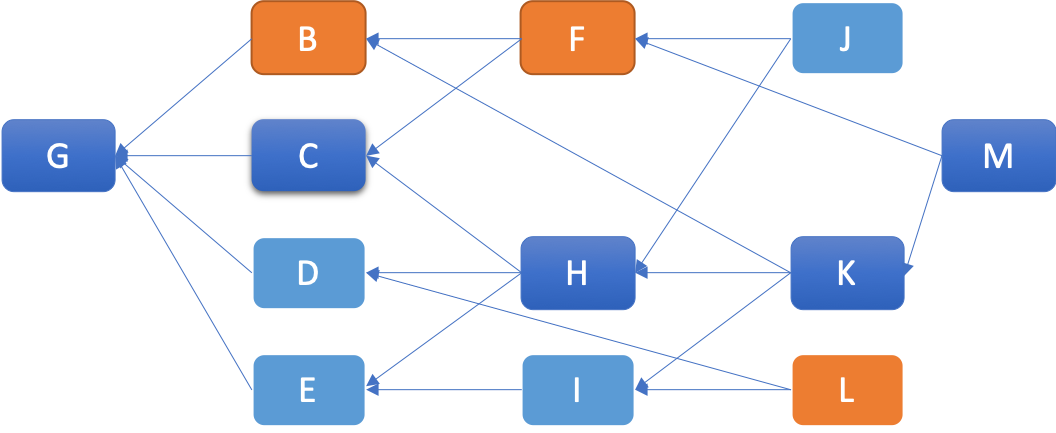
\includegraphics{figures/Ordering}}%
	}
\caption{GhostDAG 排序}
\end{figure}

例如图 5, 一个 3-集群 DAG. 

\begin{enumerate}
	\item 将 G 加入蓝色集合 
	\item 将 B,C,D,E 加入蓝色集, 因为它们的反锥体大小都小于3 
	\item 因为H的蓝色集合大于F和I的,所以在蓝色集合中加入H。在蓝色集合中加入I,因为它的反锥体大小只有2;如果反锥体尺寸大于3,则用红色标记B和F 
	\item 轮到 J, K, L;	J和K过去集合大小和蓝色集合大小都是一样的,所以目前可能有两个主链, G-C-H-J和G-C-H-K 
	\item 因为M的蓝色集合大于J和L,所以M被加入到蓝色集合中,所以只剩下一条主链,G-C-H-K-M。将因反锥体尺寸较小而产生的J加入到蓝色集合中,再将因反锥体尺寸较大而产生的F、L加入到红色集合中,现在识别出了红色集合和蓝色集合以及主链
	\item 顺序是 G-C-D-E-H-I-B-K-F-j-M-L
\end{enumerate}

\subsection{SPECTRE}

SPECTRE\cite{SPECTRE}是一种基于BlockDAG的共识协议,具有50\%的攻击承受力,实现快速确认和高吞吐量。SPECTRE只有弱活性,即只能保证对诚实的用户进行快速确认,不能保证对所有用户进行快速确认。

在活性和快速确认之间存在权衡中,SPECTRE优先选择后者,因为弱活性,只影响恶意用户,这使得SPECTRE成为一个适合支付网络的协议。如果恶意用户发起双重支付攻击,他们的交易可能会被无限期延迟。

SPECTRE是一个无状态的交易模型,因此不需要获得所有块的总排序。只有当两个块相互冲突时,才需要成对排序。SPECTRE使用投票算法来决定当两个块发生冲突时哪个块获胜。假设块 $x$有笔交易与块 $y$中的另一笔交易有冲突,并且假设块 $z$按照以下规则对它们进行投票:

\begin{enumerate}
	\item 如果$z$在$x$的未来集而不在$y$的未来集,则$z$投票支持$x$优先 $y$,表示为$x \prec y$,反之亦然。
	\item 如果$x$和$y$都在$z$的过去集中,则$z$跟过去集的多数票一致。
	\item 如果$x$和$y$都不是在$z$的过去,那么$z$跟其未来集多数投票一致
	\item $x$和$y$都为自己投票,除非其中一个已经在另一个的过去集合中
\end{enumerate}


下面是一个新区块(下图中的12号)如何投票的例子:

\begin{figure}[ht]
	\centerline{%
	   \resizebox{0.8\textwidth}{!}{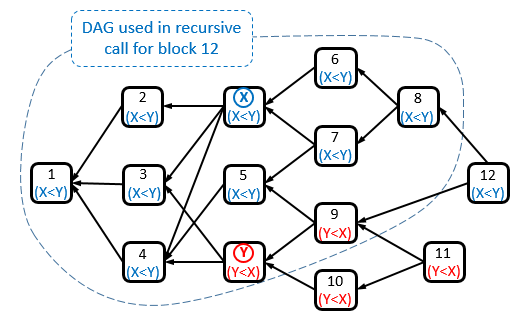
\includegraphics{figures/SPECTRE}}%
	}
\caption{DAG中对SPECTRE中的块$x$和$y$的投票过程}
\end{figure}

根据规则4,区块$x$ 投票$x \prec y$,区块$y$ 投票 $y \prec x$。

根据规则 1, 区块 6, 7 和 8 投票 $x \prec y$, 区块 9, 10 和 11 投票 $y \prec x$.


根据规则2,区块12 根据它的过去集合投票。因为不是它的过去集合中的所有区块已经投票,我们改变全局视图到区块12本地视图,
意味着第10块和第11块不包括在内


根据规则3,第5块投票为$x \prec y$,因为它未来集合的大多数投票赞成$x$ / $y$(区块7、8对区块9)。请注意
当前视图是块12的本地视图,块11被排除,所以我们不能参考它投票。

Also according to rule 3, blocks 1\textasciitilde4 vote for $x \prec y$.
同样根据规则3,块1\textasciitilde4 投票给$x \prec y$。


现在,区块12过去集合的所有区块都投票了。块$x$获得10票。块$y$得到2票。块12跟大多数走,因此投票赞成$x \prec y$。


\subsubsection*{确认时间}


当一个节点$v$接收到一个块$x$时,它将循环计算该块的风险。当风险小于给定的阈值$\epsilon$时,它接受该块。节点$v$中的$x$块的确认时间为$v$收到$x$到$v$接受$x$为止的时间。

下面的算法以$G_t^v$计算$x$块的风险,其中$G_t^v$是$v$在$t$时刻观察到的区块图

\begin{codebox}
\Procname{\proc{Risk}$(G_t^v, x)$}
\li \If $time\_now < publication(x)$
\li   \Then
        \Return 1
      \End
\li $T \gets time\_now - received^v(x)$
\li $G_x \gets G_{received^v(x) + 2 \cdot d} \cup future(x, G_t^v)$
\li $g \gets \min_{x' \in \overline{ainticone}(x,G_x)} |future(x',G_x)|$
\li \Return $risk\_hidden(T,g)$
\end{codebox}

The formula $risk\_hidden(T,g)$ is defined as:

$$
risk\_hidden(T,g) := \sum_{l=0}^{\infty} \pi(l) \sum_{m=0}^{\infty} Poiss((T + 2
\cdot d) \cdot \alpha \cdot \lambda, m) \cdot \left(\frac{\alpha}{1 -
\alpha}\right)^{(g - l - m)^+},
$$

where

\begin{itemize}
	\item $d$是网络中最近的延迟的上界,
	\item $\alpha$是攻击者的相对算力,
	\item $\lambda$ 是出块率,
	\item $Poiss(a, b)$ 被定义为 $e^{-a} \cdot \frac{a^b}{b!}$,
	\item $x^+$ 被定义为 $\max\{0, x\}$,
	\item  $\pi$ 是我们将在下面解释的平稳分布。.
\end{itemize}

$risk\_hidden(T,g)$  限定了 区块$x$ 被有偏序关系的攻击区块 $y$ 反超的概率  ,其中$y$在$x$之后发布。


$\pi$实际上是一个向量。非行式化地说,它是自区块 $x$发布以来,攻击者节点所创建的块数比诚实节点所创建的块数多多少的统计分布,在SPECTRE的论文中称为gap。$\pi(l)$是gap值为$l$的概率。

间隙值gap随着时间的推移而变化,随机游走从而形成遍历马尔可夫链。理论上,它可以是从负无穷到正无穷的任何整数。在最坏的情况下,它总是非负的。只有当差距是非负的时候,区块 $x$才有可能比某个在$x$之后发布攻击者的区块 $y$获得更少或相等的票数,导致$y$的成对排序在$x$之前。这就是为什么在$risk\_hidden$的公式中,索引$l$,即gap的值,一开始等于0,而不是负无穷。

由于$l$的随机游走引入了一个遍历马尔科夫链,$l$有一个唯一的平稳分布,即$\pi$。为了计算$\pi$,我们需要计算随机游走的转移概率矩阵。

假设$l$的值在0到$n$之间,其中$n$在上述定义中为无穷大。
我们将转移概率矩阵定义为一个$N$×$N$矩阵$T$。
用  $\delta := \alpha \cdot \lambda \cdot d$ 表示.
对所有 $1 \leq l < N - 1$, $T_{l-1,l} = 1 - \alpha, T_{l+1,l} = \alpha$, $l = N
- 1$: $T_{l-1,l} = 1 - \alpha, T_{l,l} = \alpha$
矩阵的第一列被定义为:$T_{0,0} := (1 - \alpha) \cdot e^{-\delta}, T_{1,0} = e^{-\delta}
\cdot \alpha + e^{-\delta} \cdot \delta$
对 $1 < l < N - 1$: $T_{l,0} =e^{-\delta} \cdot \frac{\delta^l}{l!}$
以及 $T_{N-1,0} = 1 - e^{-\delta} \cdot \left[\frac{\delta^0}{0!} + \frac{\delta^1}{1!} + \cdots + \frac{\delta^{N-2}}{(N-2)!}\right]$
$\pi$是$T$对应于特征值1的特征向量,其中$\pi(l) \geq 0$, $\pi$的和为1。

在实践中,当$l$非常大时,$\pi(l)$非常接近于0,所以我们可以选择$N \gg 1$而不是无穷大。因此,$risk\_hidden$的公式为

$$
risk\_hidden(T,g) = \sum_{l=0}^{N} \pi(l) \sum_{m=0}^{\infty} Poiss((T + 2 \cdot
d) \cdot \alpha \cdot \lambda, m) \cdot \left(\frac{\alpha}{1-\alpha}\right)^{(g
- l - m)^+}.
$$

建议使用一些经过良好测试的马尔科夫链库来计算$\pi$被定义为:作为R中的markovchain包。

指数为$m$的级数的和似乎是无穷级数的和。然而,对于$m > g - l$,我们有$(g - l - m)^+ = 0$ 和 
$\left(\frac{\alpha}{1-\alpha}\right)^{(g - l - m)^+} = 1$.

因此,$risk\_hidden$的公式可以进一步转换为如下公式, 其中$Poiss_{cdf}$是泊松分布的累积分布函数(CDF)

\begin{align*}
risk\_hidden(T,g)
=& \sum_{l=0}^{N}\pi(l)\sum_{m=0}^{\infty}Poiss((T+2 \cdot d) \cdot \alpha \cdot \lambda, m) \cdot (\frac{\alpha}{1-\alpha})^{(g-l-m)^+} \\
=& \sum_{l=0}^{N}\pi(l) (\sum_{m=0}^{g-l}Poiss((T+2 \cdot d) \cdot \alpha
	\cdot \lambda, m) \cdot (\frac{\alpha}{1-\alpha})^{(g-l-m)} + \\
& \sum_{m=(g-l+1)^+}^{\infty}Poiss((T+2 \cdot d) \cdot \alpha \cdot \lambda, m)) \\
=& \sum_{l=0}^{N}\pi(l) ( \sum_{m=0}^{g-l}Poiss((T+2 \cdot d) \cdot
	\alpha \cdot \lambda, m) \cdot (\frac{\alpha}{1-\alpha})^{(g-l-m)} + \\
& (1 - Poiss_{cdf} ((T+2 \cdot d) \cdot \alpha \cdot \lambda, (g-l)^+))).
\end{align*}

通过转换后的公式,我们可以用数值的方式计算$risk\_hidden$。图5模拟了不同块率下的确认时间,结果显示SPECTRE可以在高于10块/秒和10\%出错率的出块率下实现5秒的确认时间,这是很理想的。

\begin{figure}[ht]
	\centerline{%
	   \resizebox{0.8\textwidth}{!}{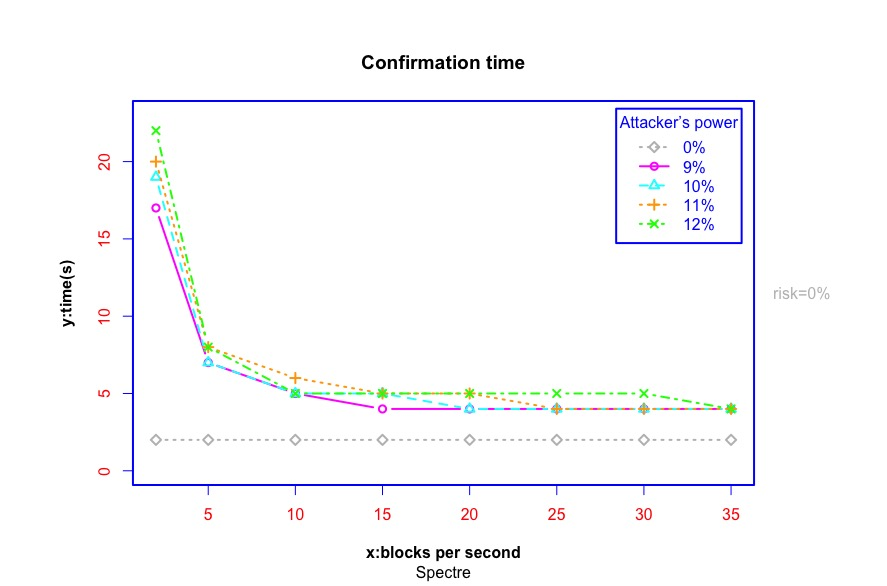
\includegraphics{figures/confirmation.jpeg}}%
	}
\caption{确认时间}
\end{figure}


\subsection{挖矿算法}

从协议的角度来看,BlockDAG的协作模型比区块链的竞争模型提供了更多的公平性。每个节点根据其贡献获得奖励,而不管它拥有多少算力。Qitmeer更倾向于公平性而不是可伸缩性,因为前者更符合区块链的真正精神。中本聪共识的意图是公平的——每个节点都用电力投票;然而,只有少数几个矿池有机会参与共识。独立矿工要付出巨大的机会成本,因为他们必须等待一段不确定的时间,在大多数情况下要等很长时间,才能开采一个区块来弥补成本;因此,它最终将不得不求助于矿坑。BlockDAG合并了每个矿工的区块,矿工有一个强烈的期望,他们的返回,然后不鼓励加入一个采矿池。

从协议的角度来看,BlockDAG的协作模型比区块链的竞争模型提供了更多的公平性。每个节点根据其贡献获得奖励,而不管它拥有多少散列能力。Qitmeer更倾向于公平性而不是可伸缩性,因为前者更符合区块链的真正精神。中本聪共识的意图是公平的——每个节点都用电力投票;然而,只有少数几个矿池有机会参与共识。独立的矿工承受着巨大的风险,因为他们必须等待一段不确定的时间,在大多数情况下是相当长的时间,才能开采一个区块来弥补成本;因此,它最终将不得不求助于矿池。BlockDAG包括每个矿工的区块,矿工对他们的回报有一个稳定的期望,因此对他们来说加入一个矿池不是太有必要。。

此外,挖矿算法是公平性的另一个因素。挖矿公平是指一定数量的挖矿成本,如在POW中产生的电量,应该得到相对等值的算力。实际上,ASIC矿机的开采效率远远高于其价格。

\subsubsection{Cuckoo-Cycle-PoW}
工作证明(PoW)用于确认交易和生成新块,并作为基于PoW的加密货币的驱动力。PoW不得使一个参与方比另一个参与方有明显的优势。这就是中本聪倡导的:“工作证明本质上是一CPU一票。”

然而,最广泛使用的工作证明算法,如SHA-256, Blake2b, Scrypt,在ASIC设备上比在CPU和GPU上更有效。这可能导致ASIC所有者拥有比CPU和GPU所有者大得多的投票权,这违反了“一CPU一票”原则。

Cuckoo-Cycle-PoW是一种基于图理论的抗ASIC工作证明算法,它被设计用来在大量伪随机生成的图中寻找某些子图。
特别地,在一个有N个节点的M条边的二分图中搜索指定长度为L的环。如果找到一个环,并且哈希难度小于目标难度,则完成布谷鸟环PoW。

\textbf{边(图)生成}


为了简单起见,我们定义了二分图为32条边。
我们两次调用SIPHASH函数来创建两个边缘端点(U和V),第一个输入值是2 * nonce,第二个输入值是2 * nonce+1。
此函数的键基于区块头的散列。

\begin{equation}
{U = SIPHASH(headerHash, 2*nonce) \mod 31}
\end{equation}
\begin{equation}
{V = SIPHASH(headerHash, 2*nonce+1) \mod 31}
\end{equation}

其中,
\begin{equation}
0\leq\ {\bf nonce} \leq 31
\end{equation} 是 0 到 31 的任意数字. 每个 nonce 对应边的两个端点(U和V).

随机在图中产生32条边:

\begin{figure}[ht]
	\centerline{%
		 \resizebox{0.8\textwidth}{!}{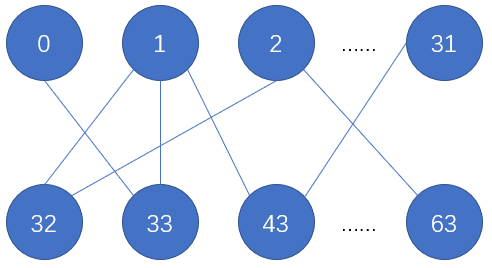
\includegraphics{figures/edge_generation}}%
	}
	\caption{产生节点.}
\end{figure}


\textbf{边裁剪}


二分图中有一条特殊的边,即叶边,它不可能是一个循环的一部分。叶边的一个特征是它所连接的节点必须至少有一个节点,节点的度为1。通过消除二分图中的叶边,可以大大降低图的复杂度,从而加快在二分图的找环的速度。

\begin{figure}[ht]
	\centerline{%
		 \resizebox{0.8\textwidth}{!}{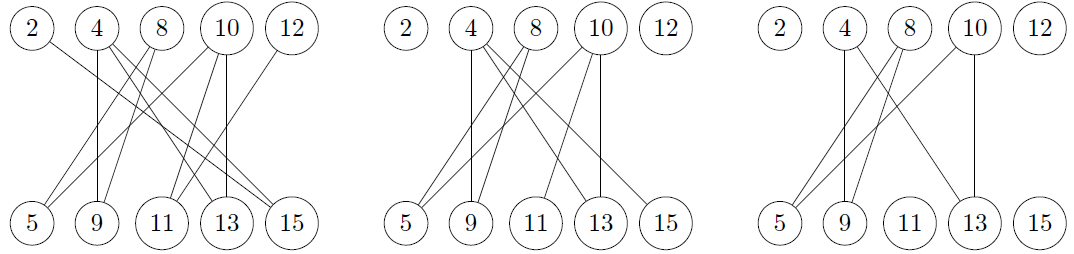
\includegraphics{figures/edge_trimming}}%
	}
	\caption{裁剪到不可能成为环的边.}
\end{figure}

\begin{itemize}
	\item 步骤1:节点0、节点3、节点10为一度节点,去掉边(0,13)、边(6,3)、边(10,9)。
	\item 步骤2:节点9和节点13为一度节点,去掉边(8,9)和边(2,13)。
	\item 步骤3:节点8是一个节点,消除边缘(8,11)。
\end{itemize}


\textbf{环检测}
经过边裁剪,如果找到一个长度为L的循环,我们认为我们已经找到了解决这个问题的方法。我们将环形边存储在一个集合中,并将生成环的nonce放入一个集合中作为返回环检测的结果。


\textbf{难度控制}
在图中找到一个环的难度与M/N成正比。这里M代表图的边数量。N表示图的节点数量。然而,在图形变化中找到一个环的难度并不大。对于加密货币,难度控制必须以精确控制的方式进行。通常的做法是M/N的比值保持不变,比如M/N = 1/2
因此在实际使用中,它也增加了类似于比特币的哈希难度控制。通过一个哈希函数获得环nonces的摘要,然后比较目标难度。

\subsubsection{难度调整}
为了保持出块率稳定,Qitmeer定时调整挖矿难度。由于BlockDAG的分叉,调整规则和区块链是不一样的

\subsubsection*{基于蓝色集}
Qitmeer调整只基于蓝色块而非所有的方块。

\subsubsection*{动态调整周期}
每个固定数量的蓝色块的难度调整是复杂的,因为不同的块有不同的蓝色集合,导致很难对哪个块是调整点达成一致。

Qitmeer利用主链来克服这个问题。规则是:

\begin{enumerate}
	\item  等待,直到比主链上的最后一个调整点后更新了144块。
    \item  计算实际时间,即从上一次调整点到现在的时间跨度。
    \item  计算新产生蓝色块的数量.
    \item  用块时间乘以这个数字计算这些蓝色块的期望时间
    \item  通过比较预期时间和实际时间来调整难度。
\end{enumerate}

\section{激励系统}

矿工为区块链网络工作的经济动力来源一个合理的激励制度。Qitmeer以一种完全去中心化的方式分配奖励——挖矿。Qitmeer关注所有节点之间的公平性,而不管一个节点拥有多少算力。对于算力强的矿工,他们可能会争取区块奖励,区块奖励比较丰富,但竞争比较激烈;对于那些算力较小的矿工,他们仍然有机会分享交易费用,先到先得。

\subsection{区块奖励}
矿工创建一个块,包括所有未经确认的交易,并生成一笔交易转一笔全网公认的资金给自己,然后找到密码学的解决方案并将其传播到网络。这就是挖矿的工作原理,这笔自我转账被称为币基(CoinBase)奖励或区块奖励。

区块奖励是相当可观的,激励矿工为获取区块而激烈竞争。BlockDAG范式是一种协作模式,因此,门槛可以更低,分配更公平,然而,块奖励本质上是一个稀缺资源,需要矿工有相当大的算力参加这个游戏. 

\subsection*{只基于蓝色集}
如共识协议部分所阐明的,GhostDAG协议用蓝色表示诚实块,用红色表示不诚实块。Qitmeer只给蓝色的方块奖励,原因如下。

\subsubsection*{鼓励矿工积极工作}
网络是依靠矿工们努力工作来巩固安全的。
BlockDAG模式的竞争不像区块链那么激烈,因此我们需要鼓励矿工积极工作,以更好地保护网络。
由于消极地工作被认定为“红块”的概率较高,矿工将努力避免这种情况

\subsubsection*{抵御潜在攻击}
包含分叉使得BlockDAG比区块链更具包容性。然而,这将降低执行攻击的成本,因为即使失败的块也将包括在账本中。因为失败的方块很可能被识别为红色方块,并且不需要支付任何费用,这就大大增加了攻击的成本,攻击者会更加谨慎地进行攻击。

\subsection{交易费}

只基于蓝色集策略可以在很大程度上增强安全性,但同时也会给那算力较弱或网络连接较差的矿工带来歧视。也许他们也是诚实的矿工,但由于共识协议的限制,他们仍然被认为是“不诚实的”。因此,我们可以利用交易费来补偿这些诚实的矿工。

\subsubsection{所有块都有交易费}
区块奖励针对的是安全性,而交易费用则更多地针对底层服务 —— 价值转移。因此,交易费的奖励政策更关心公平性,如果你为网络服务,无论你有多少算力,网络都会相应地支付给你报酬。


与区块奖励只针对蓝色区块不同,每个区块都会产生交易费,即使标记为红色。因此,矿工只要努力工作就能得到报酬。例如,由于地理位置的关系,矿工优先将地理位置接近的交易包括在内。因此,即使他们的块由于网络连通性不好而传播速度变慢,并最终被标记为红色,他们仍然可以获得交易费。

\subsubsection{加权交易费}

由于区块提异步交,BlockDAG协议不可避免地包含重复的交易,称为交易碰撞。矿工倾向于包含用更高的费用的成交易,以实现利润最大化。这将导致块的高重复率, 重复的交易不会增加吞吐量。在完全去中心化的网络中,节点之间无法相互协调以避免冲突,只有设计完善的激励机制来惩罚自私的挖矿行为。

解决这一挑战最直观的方法是分摊交易费用,这种方法会使所有的参与者达到纳什均衡,所有的参与者都会从他们的内存池中随机选择交易。这种方法将大大减少交易冲突; 然而,用户将不再支付更高的费用来提高他们的交易确认,因此该策略将破坏交易费的功能。


受到Inclusive协议的启发,Qitmeer采用了更简单的加权交易费用策略来平衡功能和碰撞。策略很简单,交易越高,相应的被包含的概率也就越高。例如,如果一个交易费用是另一个交易费用的2倍,那么从内存池中选择交易费用的可能性就是2倍。

\subsubsection{先到先得}

受到包含协议的启发,Qitmeer对交易费用采取先到先得的政策。这个想法很简单,谁第一个包含交易,谁就赢得交易费。


然而,这一想法的实施并不像预期的那么容易,也没有包含在包容性文件中。按照比特币的范式,矿商在coinbase也收取交易费,在这个阶段,它的顺序是不确定的。简单地说,矿工不知道哪个交易将是第一个包括在内,唯一的方法是假设所有的交易将是第一个,并收取所有的费用,但实际上其中一些将被认定无效。


对于这个问题,Qitmeer的解决方案是在矿工试图使用挖矿奖励时时平衡这笔交易。例如,如果一个矿工创建了一个块,其中包含3个交易,交易费均为0.1MEER,最后确定的3个交易中有2个首先被包含,其余的则不包含。当矿工创建一个交易来使用这个区块奖励时,他必须添加一个指向一个特殊地址的输出,其中包含金额0.1MEER,以消耗多余的交易费。

\section{协议与互操作}
区块链是去中心的金融系统的数字基础设施,在逐渐成熟的过程中,它将演变成一个完整的生态系统。本部分分析了在Qitmeer网络上可用的典型应用程序以及与Qitmeer交互的协议。

\subsection{挖矿算法}
\subsubsection{工作量证明算法}


设计精妙的挖矿协议能有效地抵抗了算力的集中化。
因此,Qitmeer使用了一种名为Cuckoo Cycle\cite{cuckoocycle}的工作证明算法,
该算法主要用于寻找大型伪随机图中的某些子图, 需要高强度对内存运算。

Qitmeer工作证明的介绍可以在这里\cite{qitmeerpow}找到。



\subsubsection{挖矿协议}

\begin{figure}[ht]
	\centerline{%
		\resizebox{0.8\textwidth}{!}{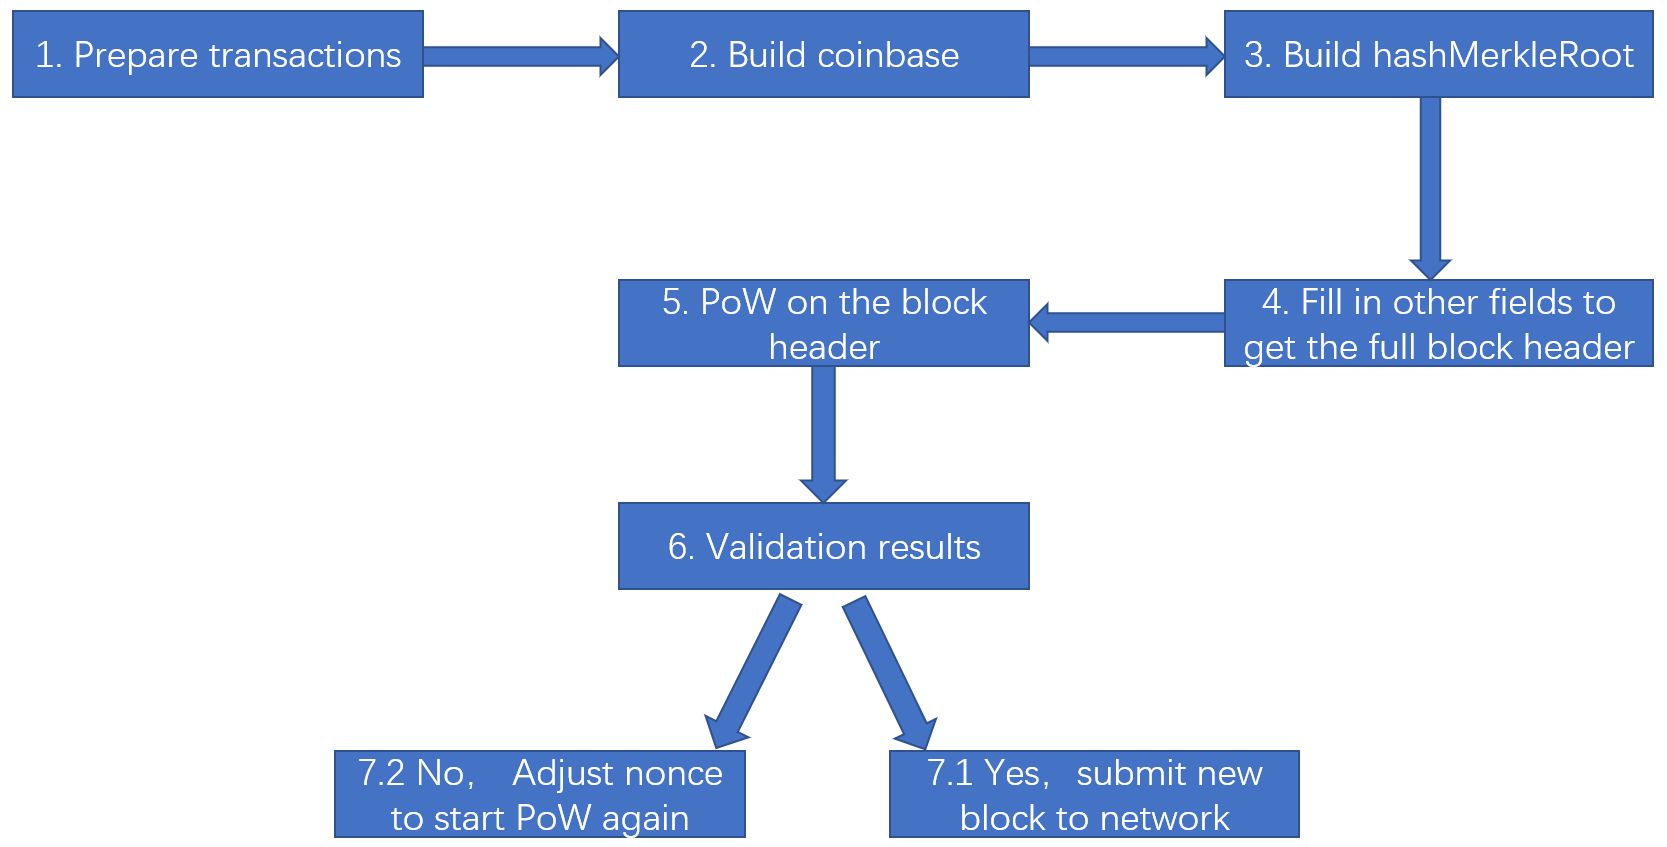
\includegraphics{figures/mining_process}}%
	}
	\caption{挖矿流程.}
\end{figure}


Qitmeer支持getblocktemplate挖矿协议。
它让矿工决定将哪些交易放到块中。
矿工通过getblocktemplate RPC向Qitmeer 全节点发送请求。

\begin{lstlisting}
{
	"jsonrpc": "2.0",
	"method": "getBlockTemplate",
	"params": [
				[
					"'$capabilities'"
				]
			],
	"id": 1
}
\end{lstlisting}
getblocktemplate 返回  JSON 对象.
\begin{lstlisting}
{
	"jsonrpc": "2.0",
	"id": 1,
	"result": {
		"bits": "207fffff",
		"stateroot": "0000000000000000000000000000000000000000000000000000000000000000",
		"curtime": 1567323822,
		"height": 6,
		"previousblockhash": "50474e0a6f88f2f1aee7a0134a7be4b6e5ab6a7c9ba440b6c11c54494ca89d32",
		"sigoplimit": 80000,
		"sizelimit": 1310720,
		"weightlimit": 4000000,
		"parents": [
		{
		"data": "329da84c49541cc1b640a49b7c6aabe5b6e47b4a13a0e7aef1f2886f0a4e4750",
		"hash": "50474e0a6f88f2f1aee7a0134a7be4b6e5ab6a7c9ba440b6c11c54494ca89d32"
		}
		],
		"transactions": [],
		"version": 4,
		"coinbaseaux": {
		"flags": "092f7169746d6565722f"
		},
		"coinbasevalue": 45000000000,
		"longpollid": "50474e0a6f88f2f1aee7a0134a7be4b6e5ab6a7c9ba440b6c11c54494ca89d32-1567323822",
		"target": "7fffff0000000000000000000000000000000000000000000000000000000000",
		"maxtime": 1567331022,
		"mintime": 1567323743,
		"mutable": [
		"time",
		"transactions/add",
		"prevblock",
		"coinbase/append"
		],
		"noncerange": "00000000ffffffff",
		"capabilities": [
		"proposal"
		]
	}
}
\end{lstlisting}


然后矿工使用来自getblocktemplate RPC的数据启动PoW。如果它得到正确的“答案”,通过submitblock RPC提交潜在的块。

\begin{lstlisting}
{
	"jsonrpc": "2.0",
	"id": 1,
	"method": "submitBlock",
	"params": [
	"data"
	]
}
\end{lstlisting}

\subsubsection{Miner 功能}

Qitmeer挖矿工具(Qitmeer-Miner) 支持独立采矿和矿池采矿。

\subsubsection*{独立模式(Solo)}
如果矿工决定在不加入池的情况下挖Qitmeer,他将启动独立挖矿模式。Solo 矿工连接一个全节点,调用RPC服务来挖块。Solo 矿工推荐使用GPU实现,以获得更高的效率。

\subsubsection*{矿池模式(Pool)}
For example:

Qitmeer矿池与大多数PoW矿池一样支持stratum挖矿协议。
例如

\emph{miner.exe -o stratum+tcp://服务器地址:3177 -m 钱包地址.机器ID}

\subsection{钱包}
\subsubsection{概述}
   区块链钱包本身不存储任何数字货币,它主要是一个用于创建数字货币交易、跟踪余额和使用户易于管理地址和私钥的计算机程序。钱包软件是整个区块链生态发展的基础,任何行业服务都可以通过一个区块链钱包的价值来实现,区块链技术本身将以自己的方式重构传统的互联网商业模式。

\subsection*{开放性}
   一个优秀的区块链公链项目应该更具包容性和开放性。因此,除了自己的官方钱包,Qitmeer在开发之初就设计了第三方钱包开发的所有接口和SDK。第三方钱包机构可以使用这些接口来开发各种支持Qitmeer令牌交易的钱包程序。包括:HD(Hierarchical Deterministic, 层级确定性)钱包,SPV(Simplified Payment Verification, 简化支付验证)钱包,浏览器钱包,满足各种用户需求。
\subsection*{怎样创建钱包}
   如下为一个简单的创建钱包的步骤
\begin{enumerate}
	\item  生成种子.
    \item  生成私钥.
    \item  生成公钥.
    \item  生成地址.
    \item  监控输出.
    \item  生成一笔未签名的交易.
    \item  对交易签名.
    \item  广播.
\end{enumerate}

   为了完成上述操作,我们需要依赖qitmeer的qitmeer SDK和RPC接口。
Qitmeer SDK是一组集成了各种加密、解密和签名功能的工具。RPC是一个基于http的网络接口,它很容易与qitmeer网络交互。
我们可以使用Qitmeer SDK来开发以下功能:

   \begin{enumerate}
    \item  得到区块数量.
    \item  通过高度得到区块信息.
    \item  查询交易信息.
    \item  得到所有待确认的交易.
    \item  监控输出.
    \item  广播交易.
   \end{enumerate}


\subsection{跨链}

Qitmeer致力于全球普惠和伦理金融的流动性通证化以及应用生态构建。因此,Qitmeer的设计目标是建立一个简单而健壮的基于UTXO模型的价值传输网络,该网络更倾向于使用链间互操作性解决方案来集成各种区块链和应用程序,比如智能合约。最终,它们将成为Qitmeer生态系统的一部分,并可以交互

\subsubsection{UTXO 互操作性}
目前,Qitmeer已经通过哈希锁定支持P2SH脚本合约和跨链功能

\subsubsection*{流程 (BTC 到 MEER)}

跨链哈希锁的实现过程为:

\begin{enumerate}
	\item  Alice和Bob分别在'MEER'和'BTC'链上生成地址;

	\item Alice 生成她的 \textit{私钥} and \textit{私钥哈希};

	\item Alice将她的'MEER'锁在'MEER'主链的哈希锁合约中。解锁条件是Bob持有\textit{私钥}或超过指定时间后返回给Alice;

	\item Bob在'MEER'中检查Alice的主链的合约,并使用\textit{私钥哈希}在'BTC'中生成相应的合约。解锁条件是Alice持有\textit{私钥}或在指定时间后返回给Bob;

	\item Alice使用\textit{私钥}从哈希锁合约中获取Bob锁定的'BTC';

	\item 获取\textit{私钥}后,Bob从哈希锁约中获取Alice锁定的'MEER',完成交易;
\end{enumerate}

\begin{figure}[hbt]
	\centerline{%
	   \resizebox{0.8\textwidth}{!}{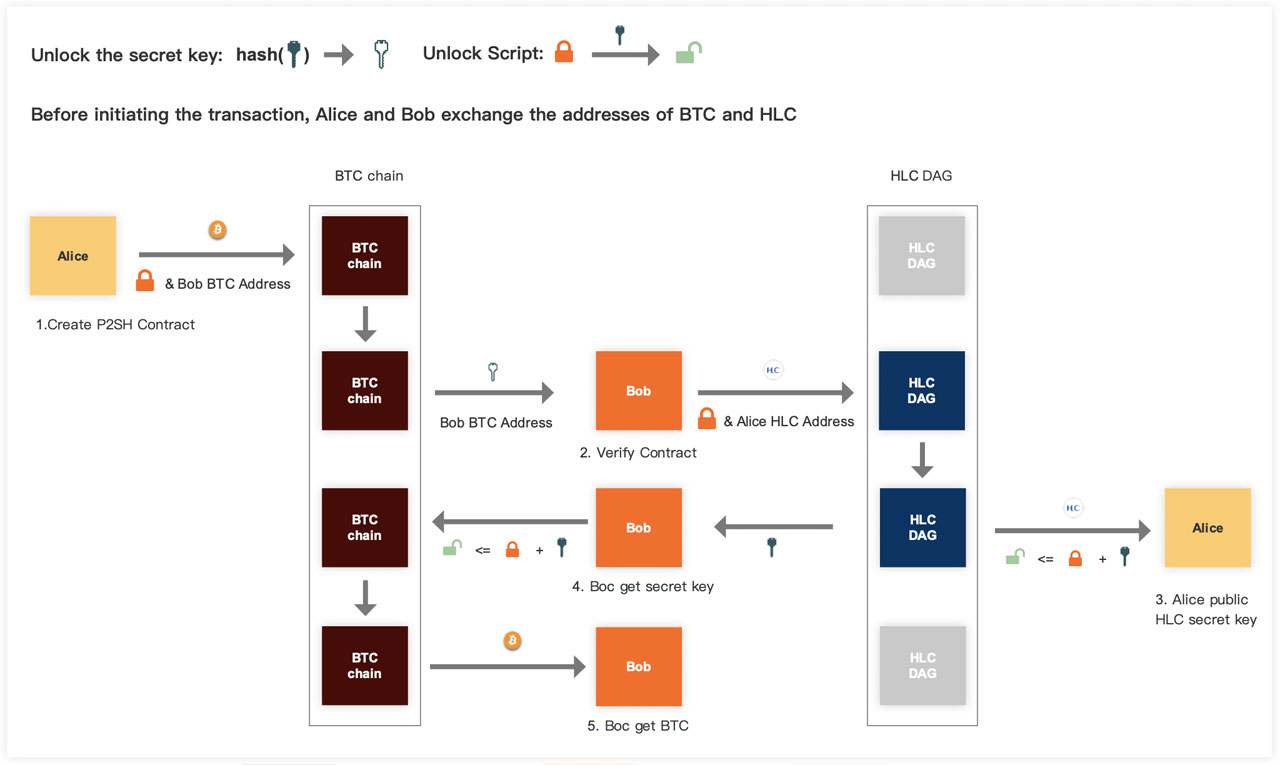
\includegraphics{figures/UTXOAtomicSwap.jpg}}%
	}
\caption{UTXO 原子交换}
\end{figure}



\subsubsection{智能合约互操作性}

Qitmeer通过哈希锁合约智能合约完成Qitmeer的区块链资产与其他账户模型之间的跨链交易。

\subsubsection*{智能合约互操作性过程 (ETH 到 MEER)}

\begin{enumerate}
	\item  Alice和Bob分别在'MEER'和'ETH'链上生成地址;

	\item Alice 生成她的 \textit{私钥} and \textit{私钥哈希};

	\item Alice将她的'MEER'锁在'MEER'主链的哈希锁合约中。解锁条件是Bob持有\textit{私钥}或超过指定时间后返回给Alice;

	\item Bob在'MEER'中检查Alice的主链的合约,并使用\textit{私钥哈希}在'ETH'中生成相应的合约。解锁条件是Alice持有\textit{私钥}或在指定时间后返回给Bob;

	 \item  Alice 使用 \textit{私钥} to 调用 智能合约 去取出 'ETH';

	\item 获取\textit{私钥}后,Bob从哈希锁约中获取Alice锁定的'MEER',完成交易;

\end{enumerate}


\clearpage
%\appendix
%\section{Appendix}
%\begin{appendices}
%\section{append A}

%Foo bar Foo bar Foo bar Foo bar Foo bar Foo bar Foo bar Foo bar Foo bar Foo bar

%\end{appendices}

%\bibliographystyle{plainnat}
%\bibliographystyle{unsrt,acm}
\bibliographystyle{unsrt}
\bibliography{qitmeer_whitepaper_cn}

\end{document}

